\section{Data Collection Performance}
\label{evaluation-sec-performance}

In this section we assess the performance of the Fetch data collection
protocol. We evaluate Fetch in terms of its \textit{yield}, its ability to
successfully collect requested data; and its \textit{latency}, the time to
download events from the network.

\subsection{Data Yield}

We define the \textit{event yield} of a Fetch transfer as the fraction of
nodes for which the entire 60~s signal was successfully downloaded following
an event. The calculation only considers those nodes that were active at the
time of the event detection (Figure~\ref{evaluation-fig-nodesalive}). For
example, if 10~nodes were active during an event, then the event yield is
defined in terms of 10~nodes. Note that the Fetch protocol attempts to
download a signal from all active nodes, even those that did not detect the
event.

\begin{figure}[t]
\begin{center}
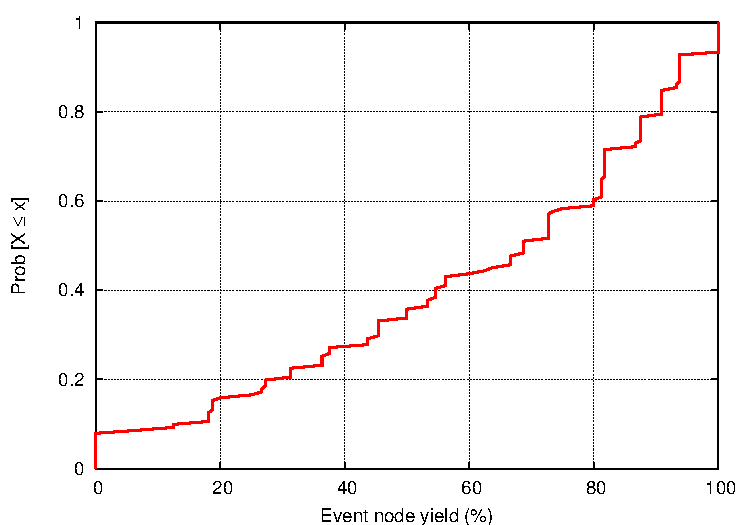
\includegraphics[width=\hsize]{./3-evaluation/figs/eventyield.pdf}
\end{center}

\caption{\textbf{Event yield.} This graph shows a CDF of the event yield for
each of the 229~events recorded during the entire deployment. Event yield is
the fraction of active nodes from which a complete 60~s signal was downloaded
following an event.}

\label{evaluation-fig-eventyield}
\end{figure}

Figure~\ref{evaluation-fig-eventyield} shows a CDF of the event yield for all
229~events recorded during the deployment. As the figure shows, the median
event yield was 68.5\% and the 90th percentile was 94\%. The yield can be
affected by several factors. First, the protocol will abort a transfer from a
node after re-requesting the same block more than 20~times, or if the
transfer from a single node exceeds 10~minutes. Second, because sampling is
disabled while performing a data transfer, if two back-to-back events occur a
node may not end up storing data for the second event.

Next, we look at the \textit{node yield} which we define as the probability
that an event was successfully downloaded from a given node. Like the event
yield, the calculation only considers those nodes that were active at the
time of each event detection. Node yield can be affected by several factors.
The depth and radio link quality of a node's routing path to the base station
affect packet loss rate and thereby the likelihood of a Fetch timeout.
Additionally, two nodes outfitted with triaxial seismometers (Nodes~250 and
251) sample and store twice as much data as the others, increasing the
probability of a timeout. Finally, a bug in our control application caused
Node~250 to sample data continuously, even during a Fetch operation. As a
result, this node was more likely to overwrite an event stored in flash
before it could be downloaded.

\begin{figure}[t]
\begin{center}
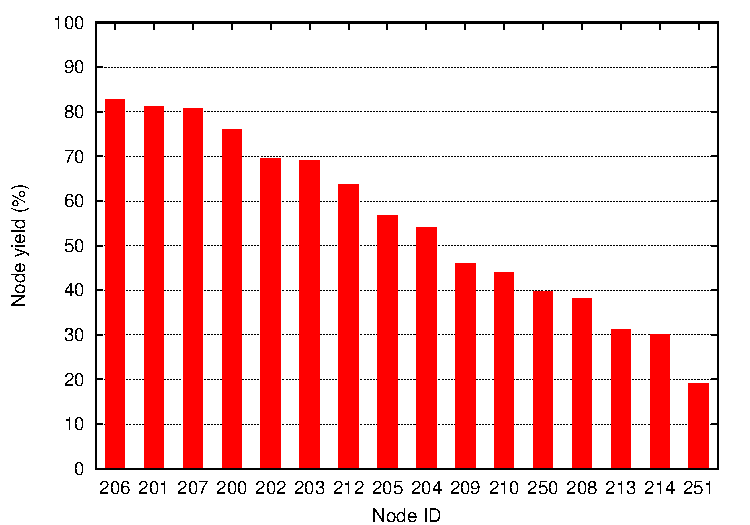
\includegraphics[width=\hsize]{./3-evaluation/figs/nodeyield.pdf}
\end{center}

\caption{\textbf{Node yield.} This graph shows the node yield for each of the
16 nodes over the entire deployment, defined as the probability that an event
was successfully downloaded from a node, as long as that node is active
during the corresponding event detection.}

\label{evaluation-fig-nodeyield}
\end{figure}

Figure~\ref{evaluation-fig-nodeyield} shows the node yield for each of the
nodes. We can see how the factors mentioned above affected performance.
First, the nodes with the highest yield (above 80\%) tend to be within two
hops from the root. However, despite being within two or three hops, Node~209
had a fairly low yield. This is explained by the fact that Node~209 had a
poor link to its closest parent, Node~200. In fact, although most nodes had a
stable parent throughout the deployment, Node~209 used Node~200 as its parent
only 33\% of the time and Nodes~206 and 207 the remaining 66\% of the time.
Node~213 also switched parents between Nodes~204 and 208, but unlike Node~209
it was always three hops away. Node~214 was the farthest node in terms of
hopcount and as a result had one of the lowest yields. The larger amount of
data was also a factor for the four-channel nodes, 250~and~251. In addition,
Node~251 was five radio hops from the gateway.


\subsection{Fetch Latency}

Transfer latency directly impacts data yield. Because we disabled sampling on
each node (apart from Node~250) during a Fetch download cycle, the duration
of the data transfer also affects a node's ability to record back-to-back
events.

\begin{figure}[t]
\begin{center}
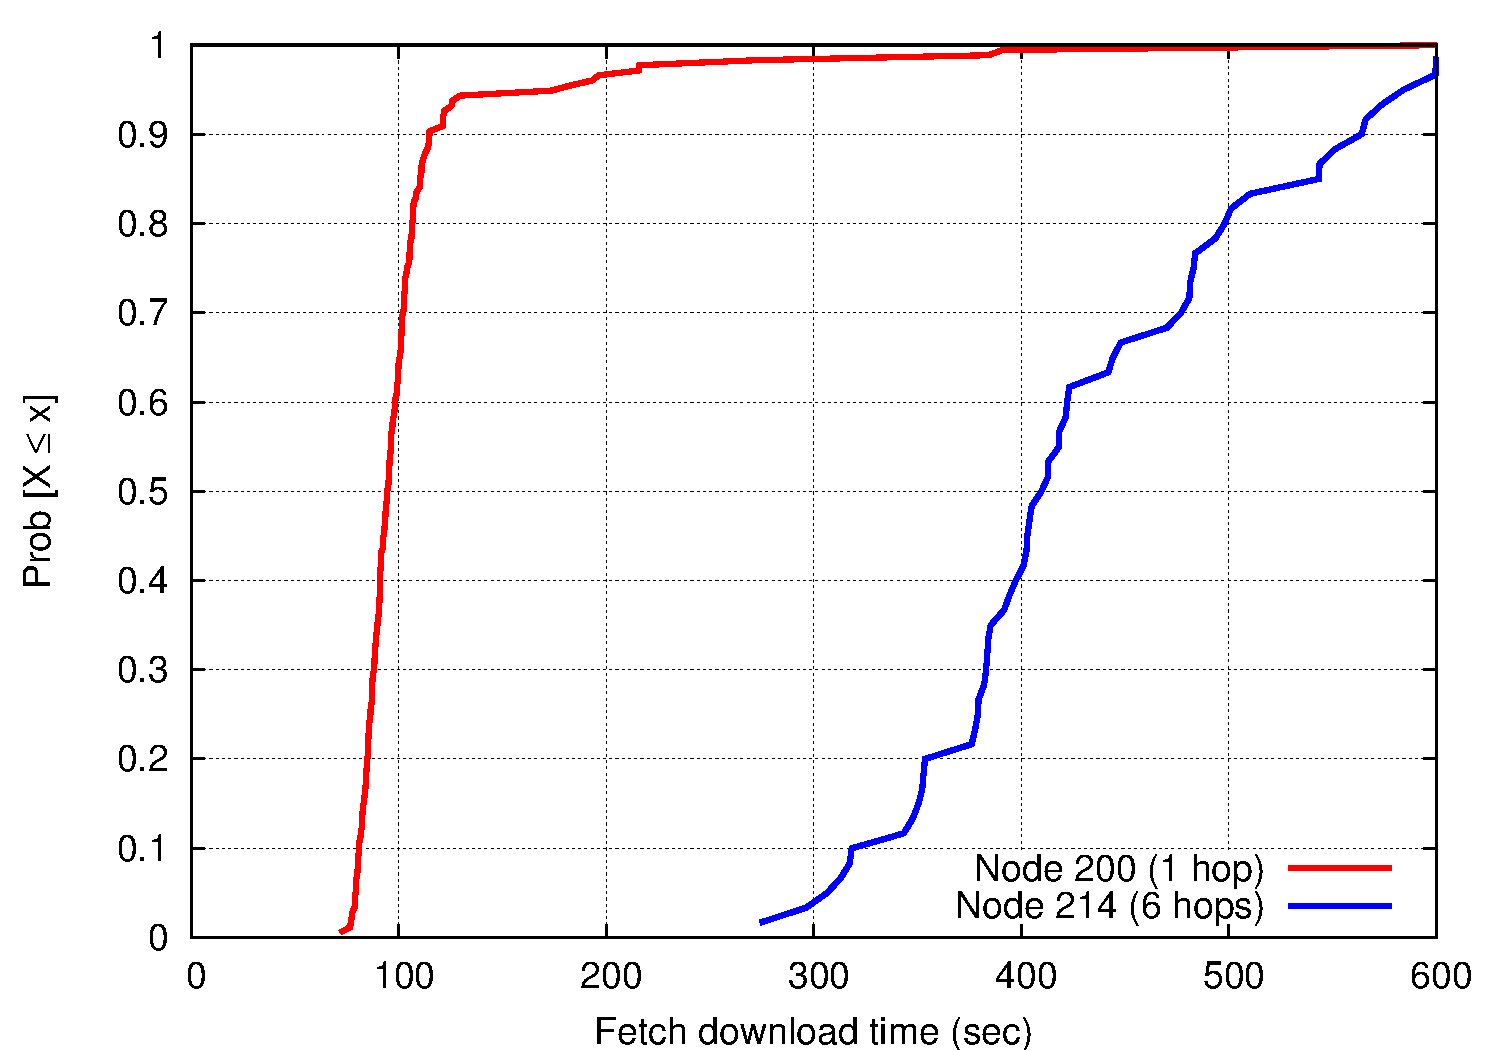
\includegraphics[width=\hsize]{./3-evaluation/figs/fetchlatency.pdf}
\end{center}

\caption{\textbf{Distribution of Fetch latency for two nodes.} The latency
for a Fetch download depends on the depth of the node in the routing tree,
which affects both command propagation latency and reliability of the routing
path. Node~200 is located 1~hop from the sink and Node~214 is located 6~hops
away.}

\label{evaluation-fig-fetchlatency}
\end{figure}

The median latency for Fetch operations (downloading 60~s worth of data from
a single node) was 186~s and the 90th percentile was 444~s. Unsurprisingly,
latency varies with the depth of the node in the routing tree.
Figure~\ref{evaluation-fig-fetchlatency} compares Fetch latency for Nodes~200
and 214, located 1~and~6 hops away from the sink, respectively. Node~200 had
a median Fetch latency of 94~s, while Node~214 had a median latency of 409~s,
about 63~s per hop. This is due to both increased delay for propagating Fetch
command messages, as well as increasing packet loss and retransmission
overheads as the data flows over multiple hops to the base.
